\documentclass[11pt, a4paper, twocolumn, twoside]{article} %ncc		
%\usepackage[sc]{mathpazo}
\usepackage[T2A]{fontenc}
\usepackage[utf8]{inputenc}
\usepackage[english, russian]{babel}
\usepackage{hyphenat}
%\hyphenation{ма-те-ма-ти-ка вос-ста-нав-ли-вать}
\usepackage{authblk}
\usepackage{indentfirst}
\usepackage{graphicx}
\usepackage{command}
\usepackage{amsmath,amsfonts,amsthm,stmaryrd,easybmat,mathrsfs,amssymb}
\usepackage{multirow}
%\usepackage[font=small,labelfont=bf]{caption}
\usepackage{color,colortbl}
\usepackage{blindtext}
\usepackage{wrapfig}

\graphicspath{ {./imgs/} }

\setlength{\parindent}{3ex}

\usepackage[hmarginratio=1:1,right=15mm,top=15mm, bottom=25mm,columnsep=20pt]{geometry}
\usepackage[small,labelfont=bf,textfont=it]{caption}
\usepackage{booktabs}
\usepackage{lettrine}
\usepackage{enumitem}
\setlist[itemize]{noitemsep}
\usepackage{abstract}
\renewcommand{\abstractnamefont}{\fontfamily{cmr}\large\bfseries} 
% Set the "Abstract" text to bold
\renewcommand{\abstracttextfont}{\normalfont\itshape} 
% Set the abstract itself to small italic text
\usepackage{titlesec} 
% Allows customization of titles
\renewcommand\thesection{\Roman{section}} 
% roman numerals for subsections
\titleformat{\section}[block]{\fontfamily{cmr}\large\scshape\bfseries}{\thesection.}{0.2em}{} 
% Change the look of the section titles
\titleformat{\subsection}[block]{\scshape\fontfamily{cmr}\bfseries}{\thesubsection.}{0.2em}{} 
% Change the look of the section titles
\titleformat{\subsubsection}[block]{\scshape\fontfamily{cmr}\bfseries}{\thesubsubsection.}{0.2em}{} 
% Change the look of the section titles
\titleformat{\paragraph}[runin]{\fontfamily{cmr}\bfseries}{2em}{}{\hspace{0ex}}

%\usepackage{fancyhdr} % Headers and footers		ДЛЯ ПРЕАМБУЛЫ
%\pagestyle{fancy} % All pages have headers and footers
%\fancyhead{} % Blank out the default header
%\fancyfoot{} % Blank out the default footer
%\fancyhead[C]{Голов~В.~А.~$\bullet$~ИММО-02-20~$\bullet$~\today} 
% Custom header text
%\fancyfoot[RO,LE]{\thepage} % Custom footer text
\usepackage{titling} % Customizing the title section
\usepackage{hyperref} % For hyperlinks in the PDF

\definecolor{DG}{RGB}{200,200,200}

\hypersetup{
    colorlinks=true,
    linkcolor=blue,
    filecolor=blue,      
    urlcolor=blue,
    citecolor=blue
}

\usepackage[margin=0pt,font=small,labelfont={rm,bf},textfont=normalfont]{caption}
\usepackage[ruled,vlined]{algorithm2e}
\newtheorem{theor}{Теорема}


%================== TRANSLATE ALGORYTHM =========================================================
\SetKwInput{KwData}{Исходные параметры}
\SetKwInput{KwResult}{Результат}
\SetKwInput{KwIn}{Входные данные}
\SetKwInput{KwOut}{Выходные данные}
\SetKwIF{If}{ElseIf}{Else}{если}{тогда}{иначе если}{иначе}{конец условия}
\SetKwFor{While}{до тех пор, пока}{выполнять}{конец цикла}
\SetKw{KwTo}{от}
\SetKw{KwRet}{вернуть}
\SetKw{Return}{вернуть}
\SetKwBlock{Begin}{начало блока}{конец блока}
\SetKwSwitch{Switch}{Case}{Other}{Проверить значение}{и выполнить}{вариант}{в противном случае}{конец варианта}{конец проверки значений}
\SetKwFor{For}{цикл}{выполнять}{конец цикла}
\SetKwFor{ForEach}{для каждого}{выполнять}{конец цикла}
\SetKwRepeat{Repeat}{повторять}{до тех пор, пока}
\SetAlgorithmName{Алгоритм}{алгоритм}{Список алгоритмов}
 

%================== TITLE SECTION =========================================================

%\setlength{\droptitle}{-7\baselineskip} % Move the title up
\pretitle{\begin{center}\fontfamily{cmr}\LARGE\bfseries} % Article title formatting
\posttitle{\end{center}}

\title{Stable-Diffusion models}

\author{Голов~В.~А.}
\affil{Конспекты по пройденному материалу}
\date{\today}

\newcommand{\fusion}[2]{#1\diamond #2}
\newtheorem{hypothesis}{Гипотеза}[section]
\newtheorem{theorem}{Теорема}[section]
\newtheorem{definition}{Определение}[section]
\renewcommand\qedsymbol{$\blacksquare$}

\begin{document}

\maketitle
\setcounter{tocdepth}{2}
\tableofcontents

\section{Модель диффузии}

\subsection{Основная идея}

Генеративная модель диффузии представляет из себя Марковский процесс, в котором прямой проход преобразует исходный объект в белый шум, то есть шум из нормального распределения. Обратным проходом модель пытается восстановить изображение из полученного ранее шума. Граф модели демонстрируется на рисунке \ref{img: 1}. 

\begin{figure*}[hbt]
  \centering
  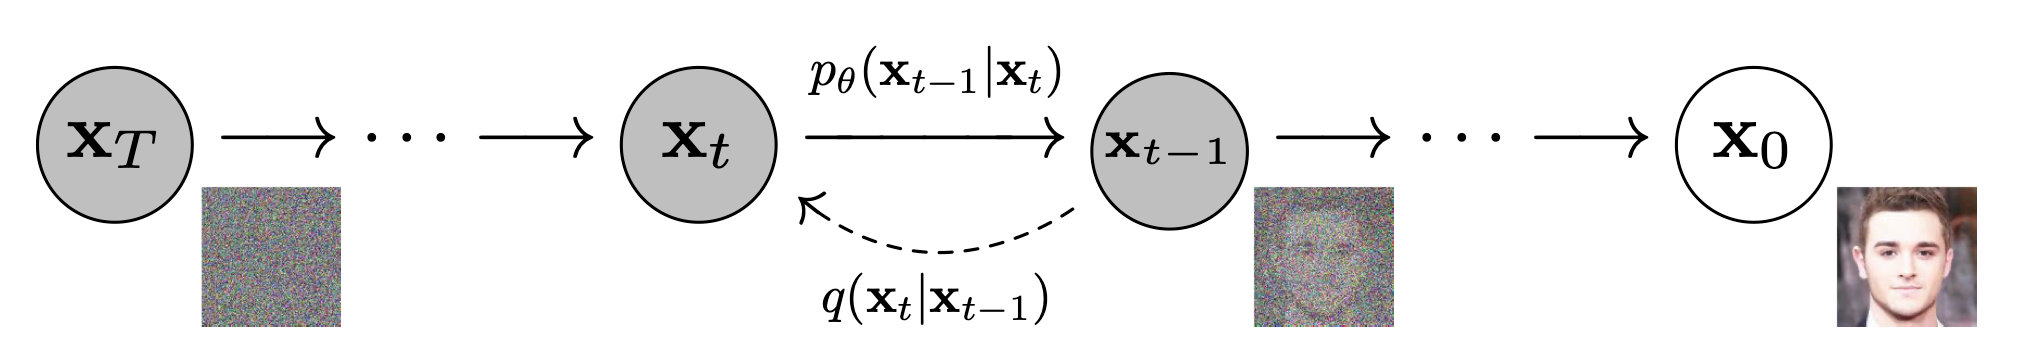
\includegraphics[width=0.8\textwidth]{imgs/1.png}
  \caption{Граф Марковского процесса, описанного в статье}
  \label{img: 1}
\end{figure*}

\subsection{Марковские цепи и их свойства}

Положим существует последовательность случайных величин $\{x_i\}_{i=0}^\infty$ и их значения $\{\xi_j\}_{j=0}^\infty$.

\begin{definition}
	Последовательность случайных величин $\{x_i\}_{i=0}^\infty$ называется \textbf{цепью Маркова}, если для любых номеров $i_1,\cdots, i_k$ и значений $\xi_{j_1},\cdots,\xi_{j_k}$ справедливо равенство 
	\begin{multline}
		P(x_{i_k} = \xi_{j_k}| x_{i_1} = \xi_{j_1},\cdots, x_{i_{k-1}} = \xi_{j_{k-1}}) = \\ = P(x_{i_k} = \xi_{j_k}| x_{i_{k-1}} = \xi_{j_{k-1}}).
	\end{multline}
\end{definition}

Другими словами, справедливо утверждение, что состояние, в котором оказалась система зависит только от последнего состояния, в котором система находилась до этого.

\begin{theorem}
	Распределение в цепи Маркова при нескольких шагах раскладывается в произведение
	\begin{equation}
		P(x_{i_k}, ..., x_{i_2}| x_{i_1}) = \prod_{t=2}^kP(x_{i_t}|x_{i_{t-1}}).
	\end{equation}
\end{theorem}
\begin{proof}
	Действительно, если воспользоваться определением условной вероятности и применим его к $i_k$, то получим
	\begin{equation*}
		P(x_{i_k}, ..., x_{i_2}| x_{i_1}) = P(x_{i_k}|x_{i_{k-1}},...,x_{i_1})P(x_{i_{k-1}},...,x_{i_2}|x_{i_1})
	\end{equation*}
	С учетом определения Марковской цепи
	\begin{equation*}
		P(x_{i_k}, ..., x_{i_2}| x_{i_1}) = P(x_{i_k}|x_{i_{k-1}})P(x_{i_{k-1}},...,x_{i_2}|x_{i_1})
	\end{equation*}
	и если продолжить последовательно раскладывать таким образом, то в итоге приходим к произведению
	\begin{equation*}
		P(x_{i_k}, ..., x_{i_2}| x_{i_1}) = \prod_{t=2}^kP(x_{i_t}|x_{i_{t-1}})
	\end{equation*}
\end{proof}

\subsection{Процесс прямой диффузии}

Положим, что у нас есть набор данных из реального распределения $x_0\sim q(x)$. Процесс прямой диффузии представляет из себя последовательное добавление за $T$ шагов небольшого гауссовского шума по планировщику разброса $\{\beta_t\}_{t=1}^T$, где $\forall t$ $\beta_t\in(0,1)$. В результате получаем последовательность зашумленных образцов $\{x_t\}_{t=1}^T$. Из определения Марковской цепи и совместного распределения следует, что 
\begin{equation}
	q(x_1,\cdots, x_T | x_0) = \prod\limits_{t=1}^Tq(x_t|x_{t-1}).
\end{equation}
Переход от $t-1$ в состояние $t$ можно описать как гауссовское зашумление
\begin{equation}
	q(x_t | x_{t-1}) = \mathcal{N}(x_t; \sqrt{1-\beta_t}x_{t-1},\beta_t I),
\end{equation}
где $I$ — единичная матрица, то есть речь идет о многомерном гауссовском распределении с диагональной матрицей ковариаций с равными значениями на ней. 

Так как многомерное гауссовское зашумление определяется как $\mathcal{N}(x; \vec\mu, \Sigma)$, где $\vec\mu$ — вектор смещения, а $\Sigma$ — матрица разброса, в нашем случае определяются как $\sqrt{1-\beta_t}x_{t-1}$ и $\beta_t I$ соответственно.

Сама операция зашумления может быть описана как
\begin{equation}
	x_t = \sqrt{1-\beta_t}x_{t-1} + \sqrt{\beta_t}\eps,
\end{equation}
где $\eps\sim\mathcal{N}(0, I)$.

Рекурентно расспишем
\begin{multline}
	x_t = \sqrt{1-\beta_t}x_{t-1} + \sqrt{\beta_t}\eps_1 = \\ = \sqrt{(1-\beta_t)(1-\beta_{t-1})}x_{t-2} + \sqrt{\beta_t}\eps_1 + \sqrt{\beta_{t-1}}\eps_2
\end{multline}
Для сложения $\sqrt{\beta_t}\eps_1$ и $\sqrt{\beta_{t-1}}\eps_2$ следует из теоремы ниже.
\begin{theorem}
	Положим есть две случайные величины $X\sim\mathcal{N}(\mu_1, \sigma^2_1)$ и $Y\sim\mathcal{N}(\mu_2, \sigma^2_2)$. Тогда случайная величина $Z=X+Y$ имеет распределение $\mathcal{N}(\mu_1 + \mu_2, \sigma^2_1+\sigma^2_2)$.
\end{theorem}
Величины $\sqrt{\beta_t}\eps_1\sim\mathcal{N}(0, \beta_t)$ и $\sqrt{\beta_{t-1}}\eps_2\sim\mathcal{N}(0, \beta_{t-1})$. Таким образом $\sqrt{\beta_t}\eps_1 + \sqrt{\beta_{t-1}}\eps_2 = \sqrt{\beta_t\beta_{t-1}} \eps^*$, где $\eps^*\sim\mathcal{N}(0, I)$. Тогда $x_t$ принимает вид
\begin{multline}
	x_t = \sqrt{(1-\beta_t)(1-\beta_{t-1})}x_{t-2} + \sqrt{\beta_t\beta_{t-1}} \eps^*.
\end{multline}
Если дальше последовательно подставить $x_{t-2},\cdots, x_1$ по аналогии получим
\begin{equation*}
	x_t = \sqrt{\prod\limits_{i=1}^{t}(1-\beta_i)}x_0 + \sqrt{\prod\limits_{i=1}^{t}\beta_i} \eps
\end{equation*}
и заменим $\alpha_t=1-\beta_t$ и $\overline{\alpha_t} = \prod_{i=1}^t \alpha_i$. Тогда выражение можно упростить
\begin{equation}
	x_t = \sqrt{\overline{\alpha_t}}x_0 + \sqrt{1-\overline{\alpha_t}} \eps,
\end{equation}
то есть
\begin{equation}
	q(x_t|x_0) = \mathcal{N}(x_t; \sqrt{\overline{\alpha_t}}x_0, (1-\overline{\alpha_t})I).
\end{equation}

Это очень приятное свойство прямого прохода, так как оно позволяет нам не проходить весь путь по цепи, а сразу насэмплировать примеры с разными уровнями шума.

\subsection{Обратный процесс диффузии}

Теперь представим, что если бы мы могли обратить процесс зашумления вспять как
\begin{equation}
	p(x_0,\cdots, x_T) = p(x_T)\prod\limits_{t=1}^Tp(x_{t-1}|x_t).
\end{equation}
Однако этого распределения мы не знаем (знаем только $p(x_T)\sim\mathcal{N}(0,I)$), поэтому будем аппроксимировать его через параметризацию $p_\theta$
\begin{equation}
	p_\theta(x_0,\cdots, x_T) = p(x_T)\prod\limits_{t=1}^Tp_\theta(x_{t-1}|x_t).
\end{equation}
Соответственно использовать для аппроксимации мы будем гауссово зашумление
\begin{equation}
	p_\theta(x_{t-1}|x_t) = \mathcal{N}(x_{t-1}; \mu_\theta(x_t, t), \Sigma_\theta(x_t, t)).
\end{equation}

\subsubsection{Обучение обратной диффузии}

В качестве обучения будем решать задачу минимизации вариационной оценки отрицательного логарифма правдоподобия (ELBO)
\begin{equation}
	\mean{}[-\log p_\theta(x_0)] \leq \mean{q}\left[-\log\dfrac{p_\theta(x_0, \cdots, x_T)}{q(x_1, \cdots, x_T|x_0)}\right],
\end{equation} 
что удачно раскладывается по формулам выше, а логарифм вносится в произведение, в результате чего получается сумма
\begin{equation*}
	\begin{aligned}
		& \mean{q}\left[-\log\dfrac{p_\theta(x_0, \cdots, x_T)}{q(x_1, \cdots, x_T|x_0)}\right] =\\
		& = \mean{q}\left[-\log\prod\limits_{t=1}^Tp_\theta(x_T)\dfrac{p_\theta(x_{t-1}| x_t)}{q(x_t| x_{t-1})}\right] = \\ 
		&= \mean{q}\left[-\log p_\theta(x_T)-\sum\limits_{t=1}^T\log\dfrac{p_\theta(x_{t-1}| x_t)}{q(x_t| x_{t-1})}\right] =: L
	\end{aligned}
\end{equation*}
Можно вынести за знак суммы член при $t=1$, а условную вероятность $q(x_t|x_{t-1})$ расписать по Байесу пользуясь определением цепей Маркова как
\begin{equation*}
	q(x_t|x_{t-1}) = q(x_t|x_{t-1}, x_0) = q(x_{t-1}| x_t, x_0)\dfrac{q(x_t|x_0)}{q(x_{t-1}|x_0)}.
\end{equation*} 
Тогда наша функция потерь принимает вид
\begin{equation*}
	\resizebox{0.5\textwidth}{!}{$
L = \mean{q}\left[-\log p_\theta(x_T)-\sum\limits_{t=2}^T\log\dfrac{p_\theta(x_{t-1}| x_t)}{q(x_{t-1}| x_t, x_0)}\cdot \dfrac{q(x_{t-1}|x_0)}{q(x_t|x_0)} - \log\dfrac{p_\theta(x_0|x_1)}{q(x_1|x_0)}\right]
$}
\end{equation*}
и преобразуем логарифм произведения в сумму логарифмов. Тогда отдельно можно рассмотреть 
\begin{equation*}
	\sum\limits_{t=2}^T\log\dfrac{q(x_{t-1}|x_0)}{q(x_t|x_0)} = \log\prod\limits_{t=2}^T\dfrac{q(x_{t-1}|x_0)}{q(x_t|x_0)} = \log\dfrac{q(x_1|x_0)}{q(x_T|x_0)}
\end{equation*}
что преобразует функцию потерь к виду
\begin{equation*}
	\resizebox{0.5\textwidth}{!}{$
L = \mean{q}\left[-\log\dfrac{p_\theta(x_T)}{q(x_T|x_0)} -\sum\limits_{t=2}^T\log\dfrac{p_\theta(x_{t-1}| x_t)}{q(x_{t-1}| x_t, x_0)} - \log p_\theta(x_0|x_1)\right].
$}
\end{equation*}
При этом логарифмы с дробями — расстояния Кульбака — Лейблера, тогда
\begin{equation}
	\resizebox{0.5\textwidth}{!}{$
L = \mean{q}\left[\underbrace{D_{KL}(q(x_T|x_0)|| p_\theta(x_T))}_{L_T} +\sum\limits_{t=2}^T\underbrace{D_{KL}(q(x_{t-1}| x_t, x_0)||p_\theta(x_{t-1}| x_t))}_{L_{t-1}}\underbrace{-\log p_\theta(x_0|x_1)}_{L_0}\right].
$}	
\end{equation}
Получается нашу функцию потерь можно расписать как сумму 
\begin{equation*}
	L = L_0 + L_1 + \cdots + L_{T_1} + L_T.
\end{equation*}

\subsubsection{Разрешимость обратной диффузии}

Покажем, что обратная условная вероятность разрешима при $x_0$. Рассмотрим $L_t$ при $0<t<T$. Для того чтобы вычислить функцию потерь сначала получим $q(x_{t-1}| x_t, x_0)$, которое пока не знаем, но, очевидно, это нормальное зашумление с неизвестными средним и дисперсией
\begin{equation*}
	q(x_{t-1}| x_t, x_0) = \mathcal{N}(x_{t-1}; \tilde{\mu}(x_t, x_0), \tilde{\beta}_tI).
\end{equation*}
Воспользуемся правилом Байеса и получим
\begin{equation*}
	q(x_{t-1}| x_t, x_0) = q(x_t|x_{t-1}, x_0)\dfrac{q(x_{t-1}|x_0)}{q(x_t|x_0)}.
\end{equation*}
Множитель $q(x_t|x_{t-1}, x_0)$ по определению Марковской цепи можно преобразовать как
\begin{equation*}
	q(x_t|x_{t-1}, x_0) = q(x_t|x_{t-1})
\end{equation*}
и тогда можно расписать плотности распределений пользуясь формулами (4) и (9) как
\begin{eqnarray*}
\begin{aligned}
	& \resizebox{0.45\textwidth}{!}{$
f(x_t|x_{t-1}) = \dfrac{1}{\sqrt{2\pi\beta_t}}\exp\left(-\dfrac{(x_t-x_{t-1}\sqrt{1-\beta_t})^2}{2\beta_t}\right);
$} \\
	& \resizebox{0.5\textwidth}{!}{$
f(x_{t-1}| x_0) = \dfrac{1}{\sqrt{2\pi(1-\overline\alpha_{t-1})}}\exp\left(-\dfrac{(x_{t-1}-x_0\sqrt{\overline\alpha_{t-1}})^2}{2(1-\overline\alpha_{t-1})}\right);
$} \\
	& \resizebox{0.45\textwidth}{!}{$
f(x_t| x_0) = \dfrac{1}{\sqrt{2\pi(1-\overline\alpha_t)}}\exp\left(-\dfrac{(x_t-x_0\sqrt{\overline\alpha_t})^2}{2(1-\overline\alpha_t)}\right);
$}
\end{aligned}
\end{eqnarray*}
С учетом того, что $\overline\alpha_t$ и $\beta_t$ являются константами и не зависят от значения $x_t$, $q(x_{t-1}| x_t, x_0)$ имеет следующую пропорцию, описанную в формуле (15). Здесь мы приводим к виду, получая квадратное уравнение (внутри экспоненты) относительно $x_{t-1}$. При этом $C(x_t, x_0)$ — некоторая функция, не зависящая от $x_{t-1}$, которую мы не расписываем по этой причине.
\begin{table*}[h!]
\begin{multline}
	q(x_{t-1}| x_t, x_0) \propto\exp\left[-\dfrac{(x_t-x_{t-1}\sqrt{1-\beta_t})^2}{2\beta_t} - \dfrac{(x_{t-1}-x_0\sqrt{\overline\alpha_{t-1}})^2}{2(1-\overline\alpha_{t-1})} + \dfrac{(x_t-x_0\sqrt{\overline\alpha_t})^2}{2(1-\overline\alpha_t)}\right] = \\ 
	= \exp\left[-\dfrac{1}{2}\cdot\left(\dfrac{x_t^2-2x_{t-1}x_t\sqrt{\alpha_t} +x^2_{t-1}\alpha_t}{\beta_t} + \dfrac{x_{t-1}^2-2x_{t-1}x_0\sqrt{\overline\alpha_{t-1}}+x_0^2\overline\alpha_{t-1}}{1-\overline\alpha_{t-1}} - \dfrac{x_t^2-2x_tx_0\sqrt{\overline\alpha_t}+x_0^2\overline\alpha_t}{1-\overline\alpha_t}\right)\right] = \\
	= \exp\left[-\dfrac{1}{2}\cdot\left(\left(\dfrac{\alpha_t}{\beta_t} + \dfrac{1}{1-\overline\alpha_{t-1}}\right)x^2_{t-1} - 2\left(\dfrac{\sqrt{\alpha_t}}{\beta_t}x_t+ \dfrac{\sqrt{\alpha_{t-1}}}{1-\overline\alpha_{t-1}}x_0\right)x_{t-1}+C(x_t,x_0)\right)\right]
\end{multline}
\end{table*}

Для простоты введем обозначения
\begin{align*}
	& A = \dfrac{\alpha_t}{\beta_t} + \dfrac{1}{1-\overline\alpha_{t-1}} \\
	& B = \dfrac{\sqrt{\alpha_t}}{\beta_t}x_t+ \dfrac{\sqrt{\alpha_{t-1}}}{1-\overline\alpha_{t-1}}x_0 \\
	& C(x_t, x_0) = \dfrac{B^2}{A}
\end{align*}
тогда выражение, описанное в (15) можно представить как
\begin{align*}
	& \exp\left[-\dfrac{1}{2}\left[Ax^2_{t-1} - 2Bx_{t-1}+\dfrac{B^2}{A}\right]\right] = \\
	& = \exp\left[-\dfrac{A}{2}\left[x^2_{t-1} - 2\dfrac{B}{A}x_{t-1}+\left(\dfrac{B}{A}\right)^2 \right]\right] = \\
	& = \exp\left[-\dfrac{A}{2}\left[x_{t-1} - \dfrac{B}{A}\right]^2\right]
\end{align*}
из чего следует, что 
\begin{align*}
	\tilde\beta_t = \dfrac{1}{A} && 
	\tilde\mu_t(x_t, x_0) = \dfrac{B}{A}
\end{align*}
При обратной подстановке искомых значений $A$ и $B$, что дисперсия равна 
\begin{multline*}
	\tilde\beta_t = \left(\dfrac{\alpha_t}{\beta_t} + \dfrac{1}{1-\overline\alpha_{t-1}}\right)^{-1} =\\= \dfrac{\beta_t(1-\overline\alpha_t)}{\alpha_t - \overline\alpha_t + \beta_t} = \dfrac{1 - \overline\alpha_{t-1}}{1 - \overline\alpha_t}\beta_t
\end{multline*}
и среднее равняется 
\begin{align*}
	& \tilde\mu_t(x_t, x_0) = \\
	& = \left(\dfrac{\sqrt{\alpha_t}}{\beta_t}x_t+ \dfrac{\sqrt{\overline\alpha_{t-1}}}{1-\overline\alpha_{t-1}}x_0\right)\left(\dfrac{\alpha_t}{\beta_t} + \dfrac{1}{1-\overline\alpha_{t-1}}\right)^{-1} = \\
	& = \left(\dfrac{\sqrt{\alpha_t}}{\beta_t}x_t+ \dfrac{\sqrt{\overline\alpha_{t-1}}}{1-\overline\alpha_{t-1}}x_0\right)\dfrac{1 - \overline\alpha_{t-1}}{1 - \overline\alpha_t}\beta_t = \\
	& = \dfrac{\sqrt{\alpha_t}(1-\overline\alpha_{t-1})}{1-\overline\alpha_t}x_t + \dfrac{\sqrt{\overline\alpha_{t-1}}\beta_t}{1-\overline\alpha_t}x_0.
\end{align*}
По формуле (8) можно вывести трансформацию $x_t$ в $x_0$ как
\begin{equation*}
	x_0 = \dfrac{1}{\sqrt{\overline\alpha_t}}(x_t - \sqrt{1-\overline\alpha_t}\eps)
\end{equation*} 
Подставив $x_0$ в $\tilde\mu_t(x_t, x_0)$ получим
\begin{align*}
	& \tilde\mu_t(x_t, x_0) =\\
	& = \dfrac{\sqrt{\alpha_t}(1-\overline\alpha_{t-1})}{1-\overline\alpha_t}x_t + \dfrac{\sqrt{\overline\alpha_{t-1}}\beta_t}{1-\overline\alpha_t}\dfrac{1}{\sqrt{\overline\alpha_t}}(x_t - \sqrt{1-\overline\alpha_t}\eps) = \\
	& = \dfrac{1}{\sqrt{\overline\alpha_t}}\left(x_t - \dfrac{1-\alpha_t}{\sqrt{1-\overline\alpha_t}}\eps\right)
\end{align*}
Получаем, что 
\begin{equation}
	\resizebox{0.47\textwidth}{!}{$q(x_t|x_{t-1}, x_0) = \mathcal{N}\left(x_t; \dfrac{1}{\sqrt{\overline\alpha_t}}\left(x_t - \dfrac{1-\alpha_t}{\sqrt{1-\overline\alpha_t}}\eps\right), \dfrac{1 - \overline\alpha_{t-1}}{1 - \overline\alpha_t}\beta_t\right).$}
\end{equation}

\subsubsection{Параметризация $L_t$ функции потерь} 

Подставим в $D_{KL}(q(x_{t-1}| x_t, x_0)||p_\theta(x_{t-1}| x_t))$ полученное нами ранее $q(x_{t-1}| x_t, x_0)$, а $p_\theta(x_{t-1}| x_t)$ выберем такое, чтобы приближать $\tilde\mu(x_t, x_0)$. В статье \cite{Ho2020} фиксируют дисперсию распределения для упрощения, при этом $\Sigma_\theta = \beta_t$ или $\Sigma_\theta = \tilde\beta_t$, что, как утверждают исследователи, на результат не влияет. Выпишем функцию потерь через плотности, взяв за дисперсию $\tilde\beta_t$.
\begin{theorem}
	$D_{KL}$ для двух нормальных распределений $p=\mathcal{N}(\mu_1, \sigma_1)$ и $q=\mathcal{N}(\mu_2, \sigma_2)$ имеет вид
	\begin{equation*}
		D_{KL}(p||q) = \log\dfrac{\sigma_2}{\sigma_1}+\dfrac{\sigma_1 + (\mu_1 - \mu_2)^2}{2\sigma_2} - \dfrac{1}{2}
	\end{equation*}
\end{theorem}
Тогда функция потерь раскладывается как 
\begin{align*}
	& L_t = \log\dfrac{\tilde\beta_t}{\tilde\beta_t} + \dfrac{\tilde\beta_t + \norm{\tilde\mu(x_t,x_0) - \mu_\theta(x_t,t)}^2}{2\tilde\beta_t} = \\
	& = \frac{1}{2\tilde\beta_t}\norm{\tilde\mu(x_t,x_0) - \mu_\theta(x_t,t)}^2 + \underbrace{\log\dfrac{\tilde\beta_t}{\tilde\beta_t}}_{C}
\end{align*}
где слагаемое $C$ можно отбросить, так как оно не зависит от $\theta$. В результате задача сводится к минимизации ошибки среднего. 

Так как нам нужно приблизить $\tilde\mu(x_t, x_0)$, которая зависит от $x_t, \alpha_t, \overline\alpha_t$, которые мы знаем, выберем в качестве $\mu_\theta(x_t, t)$ следующую функцию
\begin{equation}
	\mu_\theta(x_t, t) = \dfrac{1}{\sqrt{\overline\alpha_t}}\left(x_t - \dfrac{1-\alpha_t}{\sqrt{1-\overline\alpha_t}}\eps_{\theta}(x_t,t)\right)
\end{equation}
и подставим оба средних значения в функцию потерь
\begin{align*}
	& \resizebox{0.47\textwidth}{!}{$L_t = \frac{1}{2\tilde\beta_t}\norm{\dfrac{1}{\sqrt{\overline\alpha_t}}\left(x_t - \dfrac{1-\alpha_t}{\sqrt{1-\overline\alpha_t}}\eps\right) - \dfrac{1}{\sqrt{\overline\alpha_t}}\left(x_t - \dfrac{1-\alpha_t}{\sqrt{1-\overline\alpha_t}}\eps_{\theta}(x_t,t)\right)}^2 =$} \\
	& = \frac{(1-\alpha_t)^2}{2\alpha_t(1-\overline\alpha_t)\tilde\beta_t}\norm{\eps - \eps_{\theta}(x_t,t)}^2
\end{align*}
и вспомнив выражение (8), подставив его в $\eps_\theta$ получим конечный вид функции потерь
\begin{equation}
	L_t = \frac{(1-\alpha_t)^2}{2\alpha_t(1-\overline\alpha_t)\tilde\beta_t}\norm{\eps - \eps_{\theta}(x_t = \sqrt{\overline{\alpha_t}}x_0 + \sqrt{1-\overline{\alpha_t}} \eps,t)}^2
\end{equation}


\subsubsection{Параметризации $L_0$ и $L_T$}

Теперь рассмотрим оставшиеся два случая. Для начала рассмотрим $L_T$. 
\begin{equation*}
	L_T = D_{KL}(q(x_T|x_0)||p_\theta(x_T)) = -\log\dfrac{p_\theta(x_T)}{q(x_T|x_0)}
\end{equation*}
здесь $q(x_T|x_0)$ не зависит от $\theta$, с другой стороны $p_\theta(x_T) = p(x_T) = \mathcal{N}(0, I)$. Соответственно $L_T$ константна. В экспериментах в статье \cite{Ho2020} его определяют как $L_T\approx10^{-5}$.

С $L_0$ все интереснее
\begin{equation*}
	L_0 = -\log p_\theta(x_0|x_1)
\end{equation*}
вероятность перехода из $x_1$ в $x_0$. Так как исходное распределение содержит изображения, каждое значение которых изначально лежит в отрезке $[0, 255]$, но после нормализации приводится к отрезку $[-1, 1]$. В статье \cite{Ho2020} используется отдельный дискретный декодер, полученный из $\mathcal{N}(x_0; \mu_\theta(x_1, 1), \Sigma_\theta(x_1, 1))$, а именно
\begin{equation}
	p_\theta(x_0, x_1) = \prod\limits_{i=1}^D\int\limits_{\delta_-(x_0^i)}^{x_+(x_0^i)} \mathcal{N}(x; \mu_\theta^i(x_1, 1), \Sigma_\theta(x_1, 1))dx,
\end{equation}
где $D$ — размерность данных, а верхний индекс i указывает на извлечение одной координаты, а $\delta_-(x_0^i)$ и $\delta_+(x_0^i)$ определены как
\begin{align}
	\delta_-(x_0^i) = 
	\begin{cases}
		\begin{aligned}
			& -\infty & x=-1 \\
			& x-\frac{1}{255} & x>-1
		\end{aligned}
	\end{cases}  \\
	\delta_+(x_0^i) = 
	\begin{cases}
		\begin{aligned}
			& +\infty & x=1 \\
			& x+\frac{1}{255} & x<1
		\end{aligned}
	\end{cases}
\end{align}

\subsection{Алгоритмы обучения}

В рамках экспериментов процесс обучения выглядит следующим образом
\SetKwComment{Comment}{/* }{ */}
\begin{algorithm}
\caption{Обучение модели}\label{alg:two}
\Repeat{не покрыто}{
	$x_0 \sim q(x_0)$\;
	$t\sim\mathcal{U}[1, T]$\;
	$\eps\sim\mathcal{N}(0, I)$\;
	$\theta \leftarrow \theta - \tau\nabla_\theta\norm{\eps - \eps_\theta(\sqrt{\overline\alpha_t}x_0 + \eps\sqrt{1-\overline\alpha_t}, t)}_2^2$ \Comment{Градиентный спуск}
}
\end{algorithm}

Другими словами, речь идет о следующем:
\begin{enumerate}
  \item Сэмплируем выборку $x_0$ из реального распределения $q(x_0)$;
  \item Сэмплируем уровень шума из дискретного равномерного распределения $\mathcal{U}[1, T]$;
  \item Генерируем шум из нормального распределения и зашумляем данные (как показано выше);
  \item На основе зашумленных изображений обучаем сеть определять уровень аддитивного шума.
\end{enumerate}

Далее рассмотрим другие алгоритмы, необходимые при обучении.
\SetKwComment{Comment}{/* }{ */}
\begin{algorithm}
\caption{Сэмплирование}\label{alg:tree}
$x_T\sim\mathcal{N}(0, I)$\;
\For{$t=T,\cdots,1$}{
	\eIf{$t > 1$}{$z\sim\mathcal{N}(0,I)$ \;}{$z = \vec{0}$\;}
	$x_{t-1} = \frac{1}{\sqrt{\alpha_t}}\rb{x_t - \frac{1-\alpha_t}{\sqrt{1 - \overline\alpha_t}}\eps_\theta(x_t, t)} + z\sigma_t$\;
}
\Return $x_0$
\end{algorithm}
Алгоритм \ref{alg:tree}. использется авторами статьи \cite{Ho2020} для отслеживания прогресса. По-факту речь о том, чтобы сгенерировать шум $x_T$ самостоятельно, а затем с использованием модели привести его к $x_0$. То есть в идеале должно получиться изображение из исходного распределения $q(x_0)$. 


\bibliographystyle{abbrvurl}
\bibliography{refs.bib}


\end{document}
